
% TODO:
% memory diagrams -- diff between modifying in place and returning a copy (like
% .strip().)
% Show the "x = x + 5" pattern for computing a running total.

\chapter{Calculations}
\label{ch:calculations}

Our discipline obviously involves a lot of computation -- in fact, I expect the
first image that comes to mind when most people hear the words ``data science''
is one of numerical calculation. In this chapter, I'll lay out the Python
syntax for performing various mathematical operations on numbers, as well as
manipulating strings. These things appear in every program, and you'll find it
all straightforward.

And then I'll drop a bomb on you. I'll unveil a Python behavior which you'll
probably find completely unexpected, which flummoxes nearly every student who
first sees it, and yet which you must understand and master to succeed in
Python or any programming language.

\section{Mathematical operations}

\index{operator}

\index{bananas (parentheses)}
\index{()@\texttt{()} (bananas)}
\index{curlies (curly braces)}
\index{\{\}@\texttt{\{\}} (curlies)}
\index{boxies (square brackets)}
\index{[]@\texttt{[]} (boxies)}
\index{wakkas (angle brackets)}
\index{<>@\texttt{<>} (wakkas)}
\index{+@\texttt{+}}
\index{-@\texttt{-}}
\index{/@\texttt{/}}
\index{**@\texttt{**}}
First, the easy part. Python has a number of built-in \textbf{operators} to do
the familiar math stuff. Figure~\ref{fig:mathOps} has a table of the ones we'll
use. A few are mildly surprising (\texttt{*} instead of \texttt{X} for
multiplication; \texttt{/} instead of $\div$ for division, which I'll bet you
couldn't find on your keyboard anyway), and you have to remember to use only
bananas (not boxies \texttt{[]}, curlies \texttt{\{\}}, or wakkas \texttt{<>})
for grouping sub-expressions within a larger expression. Otherwise, it's a
piece of cake.

\begin{figure}[ht]
\centering
\begin{tabular}{c | l}
\hline
Operator & Operation \\
\hline
\texttt{+} & addition \\
\texttt{-} & subtraction \\
\texttt{*} & multiplication \\
\texttt{/} & division \\
\texttt{**} & exponentiation (``to the power of'')\\
\texttt{()} & grouping \\
\hline
\end{tabular}
\smallskip
\caption{Python's basic math operators.}
\label{fig:mathOps}
\end{figure}

All this stuff has to appear on the \textbf{right-hand side} of an equals sign,
by the way, never on the left. That may seem surprising, since in mathematics
the equations ``$x = y + 3$'' and ``$y + 3 = x$'' mean the same thing. Why does
it matter which order you write it in? The answer, you'll recall, is that in a
program the symbol ``\texttt{=}'' doesn't mean ``\textit{is} equal to'' but
rather ``\textit{make} equal to.'' It's not an equation; it's a command. And
you can't command ``$y+3$'' to be equal to anything. Therefore the only thing
permitted on the left-hand side of an equals sign is a single, plain-jane
variable name.

To test your understanding of the syntax, see if you agree that the following
math expression:

\begin{align*}
\textrm{gpa} = \frac{
\textrm{creds}_1 \cdot \textrm{gpts}_1 +
\textrm{creds}_2 \cdot \textrm{gpts}_2}
{\textrm{creds}_1 + \textrm{creds}_2}
\end{align*}

should look like this in Python:

\begin{Verbatim}[fontsize=\footnotesize,samepage=true,frame=single,framesep=3mm]
gpa = (creds1 * gpts1 + creds2 * gpts2) / (creds1 + creds2)
\end{Verbatim}

and that this one:

\begin{align*}
a = \frac{\lbrack x^2y(4-z) + (x+q)\cdot y \rbrack \times 2^{15y+2z}}
{19x^3 - (yz)^{(y-1)^2}}
\end{align*}

should look like this:

\begin{Verbatim}[fontsize=\tiny,samepage=true,frame=single,framesep=3mm]
a = (((x**2)*y*(4-z) + (x+q)*y) * 2**(15*y+2*z)) / (19*(x**3) - (y*z)**((y-1)**2))
\end{Verbatim}

\vspace{-.15in}

If so, you're good to go. It's tedious, but not complicated.

Python also has plenty of functions for absolute value, sine and cosine,
logarithms, square roots, and anything else you can think of. We'll learn all
those at the proper time (or they're all eminently Google-able if you want to
look them up now).


\section{String operations}

\index{trimming@trimming (a string)}
\index{whitespace}
\index{tacking on (concatenating) strings}
\index{concatenating!strings}
\label{concatenatingStrings}
\index{+@\texttt{+}}
\index{case@case (upper and lower)}
Text data, too, has many things that can be done to it. For now, let's just
learn a few techniques for \textbf{concatenating} strings (tacking one onto the
end of another) \textbf{trimming} strings (removing
\textbf{whitespace}\footnote{The word ``whitespace'' is a catch-all for spaces,
tabs, newline characters, and most anything else invisible.} from the ends) and
changing their \textbf{case} (upper/lower). See Figure~\ref{fig:stringOps} for
a list.

\index{lstrip@\texttt{.lstrip()}}
\index{rstrip@\texttt{.rstrip()}}
\index{strip@\texttt{.strip()}}
\index{upper@\texttt{.upper()}}
\index{lower@\texttt{.lower()}}
\index{title@\texttt{.title()}}

\begin{figure}[ht]
\small
\centering
\begin{tabular}{c | l}
\hline
Method/operator & Operation \\
\hline
\texttt{+} & concatenate two strings \\
\texttt{.lstrip()} & remove leading whitespace \\
\texttt{.rstrip()} & remove trailing whitespace \\
\texttt{.strip()} & remove leading and trailing whitespace \\
\texttt{.upper()} & convert to all uppercase \\
\texttt{.lower()} & convert to all lowercase \\
\texttt{.title()} & convert to ``title case'' (capitalize each word) \\
\hline
\end{tabular}
\smallskip
\caption{A few of Python's string methods.}
\label{fig:stringOps}
\end{figure}

The plus sign is an operator, like the mathematical ones in
Figure~\ref{fig:mathOps}: it's used to concatenate (append) one string to
another. Example:

\begin{Verbatim}[fontsize=\small,samepage=true,frame=single,framesep=3mm]
x = "Lady"
y = "Gaga"
z = x + y
print(z)
\end{Verbatim}

\begin{Verbatim}[fontsize=\small,samepage=true,frame=leftline,framesep=5mm,framerule=1mm]
LadyGaga
\end{Verbatim}

The second one is slapped right on the end of the first; there's no spaces or
punctuation. If you wanted to insert a space, you'd have to do that explicitly
with a string-that-consists-of-only-a-space (written as the three characters:
quote, space, quote), like this:

\begin{Verbatim}[fontsize=\small,samepage=true,frame=single,framesep=3mm]
first = 'Dwayne'
last = "Johnson"
full = first + ' ' + last
print(full)
\end{Verbatim}

\begin{Verbatim}[fontsize=\small,samepage=true,frame=leftline,framesep=5mm,framerule=1mm]
Dwayne Johnson
\end{Verbatim}

Punctuation marks, too, have to be included literally, and it can be tricky to
get everything typed in the right way:

\begin{Verbatim}[fontsize=\small,samepage=true,frame=single,framesep=3mm]
first = 'Dwayne'
last = "Johnson"
nick = 'The Rock'
full = first + ' "' + nick + '" ' + last
print("Don't ya just love {}?".format(full))
\end{Verbatim}

\begin{Verbatim}[fontsize=\small,samepage=true,frame=leftline,framesep=5mm,framerule=1mm]
Don't ya just love Dwayne "The Rock" Johnson?
\end{Verbatim}

Stare at that line beginning with ``\texttt{full =}'' and see if you can figure
out why each punctuation mark is where it is, and why there are spaces between
some of them and not between others.

By the way, here's a bit of a head-scratcher at first:

\begin{Verbatim}[fontsize=\small,samepage=true,frame=single,framesep=3mm]
matriculation_year = "2019"
graduation_year = matriculation_year + 4
print("Imma graduate in {}!".format(graduation_year))
\end{Verbatim}

\begin{Verbatim}[fontsize=\small,samepage=true,frame=leftline,framesep=5mm,framerule=1mm]
Imma graduate in 20194!
\end{Verbatim}

Whoa -- wut? That's a lot of tuition. The problem here is that
\texttt{matriculation\_year} was defined as a \textit{string}, not an integer
(note the quotes). So the \texttt{+} sign meant concatenation, not addition.
Remember: a string-consisting-only-of-digits is not the same as a number. (If
you remove the quotes from the first line, your mom will breathe easier and
you'll get the result you expect.)

The other items in Figure~\ref{fig:stringOps} are methods: they have an initial
dot (``\texttt{.}'') and they must be called ``\textbf{on} a string'' (meaning,
a string variable name must immediately precede them). They also take no
arguments, which means that a lonely, empty pair of bananas comes after their
name when they are called. Examples:

\index{Carl's Ice Cream}
\begin{Verbatim}[fontsize=\small,samepage=true,frame=single,framesep=3mm]
shop_title = "               carl's ICE cream      "
print(shop_title)
print(shop_title.strip())
print(shop_title.upper())
print(shop_title.lower())
print(shop_title.title())
\end{Verbatim}

\begin{Verbatim}[fontsize=\small,samepage=true,frame=leftline,framesep=5mm,framerule=1mm]
               carl's ICE cream         
carl's ICE cream
               CARL'S ICE CREAM         
               carl's ice cream         
               Carl'S Ice Cream         
\end{Verbatim}

(You can't see the trailing spaces in the output, but you can see the leading
ones.)

You can even combine method calls back to back like this:

\begin{Verbatim}[fontsize=\small,samepage=true,frame=single,framesep=3mm]
print(shop_title.strip().upper())
\end{Verbatim}

\begin{Verbatim}[fontsize=\small,samepage=true,frame=leftline,framesep=5mm,framerule=1mm]
Carl'S Ice Cream
\end{Verbatim}

\index{data cleansing}
These operations are for more than mere prettiness. They're also used for
\textbf{data cleansing}, which is often needed when dealing with messy,
real-world data sets. If, say, you asked a bunch of people on a Web-based
survey which Fredericksburg ice cream store they prefer, lots of them will name
Carl's: but they'll type the capitalization every which way, forget the
apostrophe, clumsily add spaces to one end (or even both, or even in the
middle), yet they'll all have in mind the same luscious vanilla cones. One step
towards conflating all these different expressions to the same root answer
would be trimming the whitespace off the ends and converting everything to all
lower-case. More surgical operations like removing punctuation or spaces in the
middle is a bit trickier; stay tuned.

\section{Return values}

\label{returnValues}
\index{bomb}
Okay, you've been in suspense long enough. Time for the bomb.

\index{calling a function@``calling'' a function}
\index{passing an argument@``passing'' an argument}
First, we're going to add another phrase to our already lengthy
function-calling mantra. You'll recall that we summarized this code (a function
call):

\begin{Verbatim}[fontsize=\small,samepage=true,frame=single,framesep=3mm]
len(movie_title)
\end{Verbatim}

with this English:

\begin{quote}
``We are calling the \texttt{len()} function, and passing it
\texttt{movie\_title} as an argument.''
\end{quote}

\index{calling a method@``calling'' a method (on a variable)}
\index{on@``on''}
And we summarized this code (a method call):

\begin{Verbatim}[fontsize=\small,samepage=true,frame=single,framesep=3mm]
message.format(name, age)
\end{Verbatim}

with this English:

\begin{quote}
``We are calling the \texttt{.format()} method \textbf{on} the \texttt{message}
variable, and passing it \texttt{name} and \texttt{age} as arguments.''
\end{quote}

\index{return value}
\index{output!of a function}
\index{return@``returning'' a value}
Now, a third thing. We can use the equals sign with a variable name to
capture the output of the function or method, instead of just printing it. The
output of a function is called its \textbf{return value}. We say that ``the
\texttt{.upper()} method \textbf{returns} an upper-case version of the string
it was called \textbf{on}.'' We can capture it like this:

\begin{Verbatim}[fontsize=\small,samepage=true,frame=single,framesep=3mm]
big_and_loud = shop_title.upper()
\end{Verbatim}

The variable \texttt{big\_and\_loud} now holds the value
\texttt{"CARL\textquotesingle S ICE CREAM"}. Functions work similarly:

\begin{Verbatim}[fontsize=\small,samepage=true,frame=single,framesep=3mm]
width_of_sign = len(shop_title)
\end{Verbatim}

The \texttt{width\_of\_sign} int now has the value 40 (remember all those
extraneous spaces); if we'd trimmed first, we'd have gotten 16:

\begin{Verbatim}[fontsize=\small,samepage=true,frame=single,framesep=3mm]
true_width_of_sign = len(shop_title.strip())
print(true_width_of_sign)
\end{Verbatim}

\begin{Verbatim}[fontsize=\small,samepage=true,frame=leftline,framesep=5mm,framerule=1mm]
16
\end{Verbatim}


\subsection{The bomb}

I've probably built this up too much, but I think you'll agree that the
following output is pretty surprising:

\begin{Verbatim}[fontsize=\small,samepage=true,frame=single,framesep=3mm]
diva = "Ariana Grande"
diva.upper()
print("I just love {}!".format(diva))
\end{Verbatim}

\begin{Verbatim}[fontsize=\small,samepage=true,frame=leftline,framesep=5mm,framerule=1mm]
I just love Ariana Grande!
\end{Verbatim}

Wait...did the ``\texttt{diva.upper()}'' part just not work? Did it get
skipped? Did we do it wrong somehow?

Even more confusing, putting the ``\texttt{.upper()}'' call directly in the
\texttt{print} statement seems to work...but only temporarily. Accessing
\texttt{diva} a moment later appears to revert it back to its old value:

\begin{Verbatim}[fontsize=\small,samepage=true,frame=single,framesep=3mm]
diva = "Ariana Grande"
print("I just love {}!".format(diva.upper()))
print("When does the next {} album come out?".format(diva))
\end{Verbatim}

\begin{Verbatim}[fontsize=\small,samepage=true,frame=leftline,framesep=5mm,framerule=1mm]
I just love ARIANA GRANDE!
When does the next Ariana Grande album come out?
\end{Verbatim}

The root cause of this and practically all perplexing Python printing can be
discovered by consulting the memory picture. Here's how it starts out when we
first define \texttt{diva}:

\vspace{-.2in}
\begin{center}
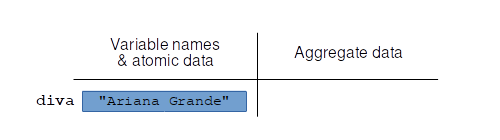
\includegraphics[width=0.9\textwidth]{bomb.png}
\end{center}

Now say we do this:

\begin{Verbatim}[fontsize=\small,samepage=true,frame=single,framesep=3mm]
new_var_name = diva.upper()
\end{Verbatim}

The result is this picture:

\vspace{-.2in}
\begin{center}
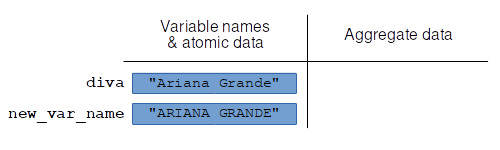
\includegraphics[width=0.9\textwidth]{bomb2.png}
\end{center}

And now we see the reason for it all. The contents of the \texttt{diva}
variable itself are \textit{\textbf{unchanged}} by the method call. Calling
``\texttt{.upper()}'' on \texttt{diva} didn't change the string value in
\texttt{diva}: it merely \textit{returned} a modified \textit{copy} of the
string.

Think of it this way: if I asked you, ``what is your name in Pig Latin?'' and
you told me, that would not intrinsically \textit{change} your actual name to
be in Pig Latin. You would simply be ``returning'' to me the Pig Latin version
of it in response to my query.

You could argue this behavior of Python's is dumb, or at best misleading, and
I'm actually inclined to agree with you in this case. But of course beggars
can't be choosers: someone took the time to write the \texttt{.upper()} method
for us, so if we want to take advantage of it we have to use his/her owner's
manual. And the fact is that many (perhaps even most) Python functions/methods
-- including many of the ones from Pandas, which we'll use extensively -- are
coded with this style: not actually modifying the variables they are passed,
but instead returning to you a modified copy which you must store.

Now given that this is the case, it would at least be nice if I could tell you
that it always, consistently worked this way. Then you could simply accept it
and get used to it. Alas, no. There \textit{are} functions/methods (lots of
them) which \textit{do} modify a parameter or the variable they were called on.
So sometimes, our na\"{i}ve approach of calling the method and expecting the
variable to change is exactly what we need to do. The bottom line is:
\textit{there's no way of knowing without being told, or else reading the
documentation.} We'll learn how to do the latter in a future chapter. For now,
I'm simply telling you for the record that the methods in
Figure~\ref{fig:stringOps} are all of the ``return a modified copy'' type, and
giving you a heads up that both styles of method do exist out there in
abundance.

A couple more things. First, as a corollary of the above, realize that the
following statement (on a line by itself) is officially 100\% useless:

\begin{Verbatim}[fontsize=\small,samepage=true,frame=single,framesep=3mm]
name_of_pet.lstrip()
\end{Verbatim}

You called the \texttt{.lstrip()} method, and then....did nothing with the
return value. If you don't store it in a variable -- or else do something with
it right away like \texttt{print} it before it slips out of your fingers --
it's irrevocably lost: it doesn't even show up on the memory picture because
there's no variable name. (Think about that.)

Second, note the following pattern which is very often used:

\begin{Verbatim}[fontsize=\small,samepage=true,frame=single,framesep=3mm]
name_of_pet = name_of_pet.lstrip()
\end{Verbatim}

Here, we're calling \texttt{.lstrip()} on the \texttt{name\_of\_pet} variable
\textit{and then storing the return value back in the \texttt{name\_of\_pet}
variable}. This might be what you thought would have happened in the first
place -- the author of the previous, useless line, probably wanted the variable
itself to permanently have its leading spaces removed. Simply calling
\texttt{.lstrip()} on the variable won't do that, but putting the revised value
back in the same blue box on the memory diagram will.
